\section{Use of the program}
\subsection{Requirements}
\begin{itemize}
	\item Mozilla Firefox version 50 or more
	\item Google Chrome version 60 or more
\end{itemize}

\subsection{Metamask installation and configuration}
Go to the site \url{https://metamask.io} . 

\begin{labeling}{alligator}
	\item If you're using Firefox, you will see a link named \textbf{GET FIREFOX ADDON}, click on it. Then click \textbf{Add to Firefox} and then click \textbf{Add} on the pop-up.
	\item If you're using Chrome, you will see a link named \textbf{GET CHROME EXTENSION}, click on it. Then click \textbf{Add} and then click \textbf{Add extension} on the pop-up.
\end{labeling}
Now in the browser: click on the MetaMask icon on the top right and accept the Privacy Notice and the Terms of use by clicking on \textbf{Accept}.

\subsection{Creation of a digital wallet}
Insert a new password (it is needed to unlock the account) and click \textbf{CREATE} (as in Figure~\ref{fig:password}).
\begin{figure}[!h]
	\centering
	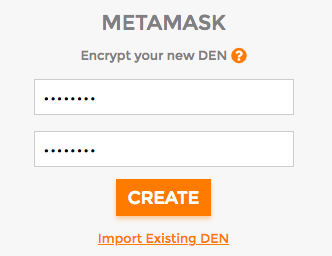
\includegraphics[height=3in]{img/password.png}
	\caption{Setting the password}
	\label{fig:password}
\end{figure}

Now store somewhere on your drive the 12 words seed phrase (an example of seed phrase is showed in Figure~\ref{fig:seed}).
\begin{figure}[!h]
	\centering
	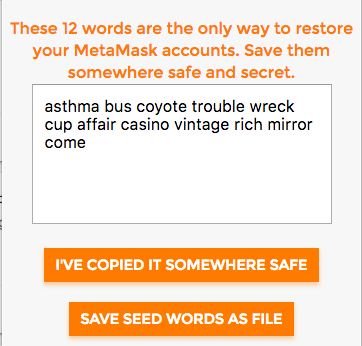
\includegraphics[height=3in]{img/seed.png}
	\caption{The seed phrase}
	\label{fig:seed}
\end{figure}


\subsection{Restore the digital wallet}
You have the possibility to restore your account if you loose the password or change the browser or even the computer. The only thing you need to do is to click on the Metamask icon and then click on \textbf{Restore from seed phrase}. Now paste inside the box the seed phrase that you have saved previously, insert a new password and click \textbf{OK}.

\subsection{Connection to the application}
\WarningSubsection{}

To use the application visit the page \textcolor{red}{	\dots}.

Now you're able to use Marvin! You should see the \project{} main page (like the one showed in Figure~\ref{fig:main}).
\begin{figure}[H]
	\centering
	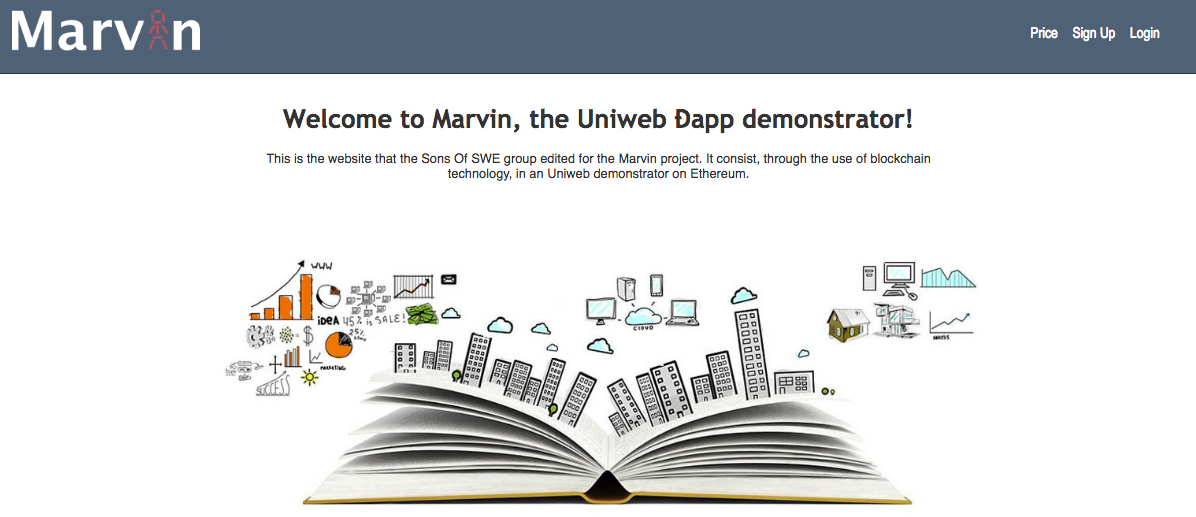
\includegraphics[width=0.9\textwidth]{img/main.png}
	\caption{The \project{} main page}
	\label{fig:main}
\end{figure}

\subsection{Operations prices}
If you are interested in seeing the costs of the operations that the site allows you  to complete, then you can click on the voice \textbf{Price}, listed in the blue bar located at the top of the screen. You will be redirect to a page like the one in Figure~\ref{fig:price}, that contains an always up to date estimation of the cost of the operations.
\begin{figure}[H]
	\centering
	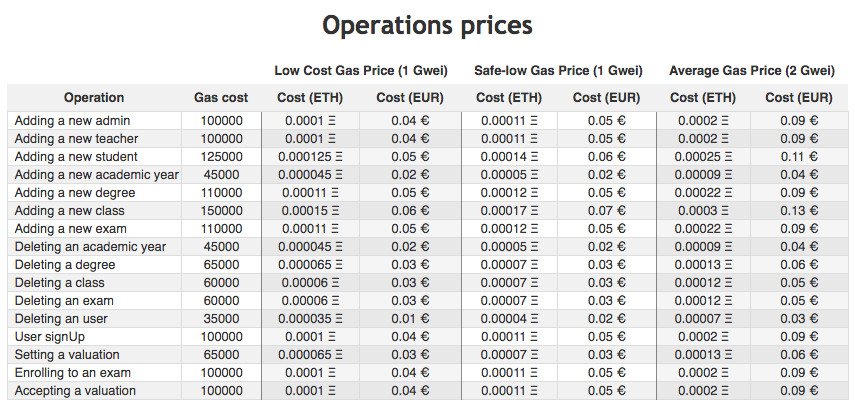
\includegraphics[width=0.90\textwidth]{img/price.png}
	\caption{The cost of the \project's operation}
	\label{fig:price}
\end{figure}
